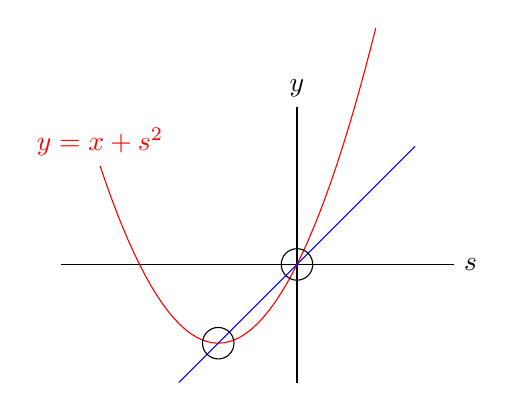
\begin{tikzpicture}
% Axis
\draw (-3,0)--(2,0) node[right]{$s$};
\draw (0,-1.5)--(0,2) node[above]{$y$};

\draw[red, samples=50, domain=-2:1.5] plot({-\x-1},{-1+\x*\x}) node[above] {$y=x+s^2$};
\draw[samples=50, domain=-1.5:1.5, blue] plot({\x},{\x});

\draw (-1,-1) circle[radius = 0.2cm];
\draw ( 0, 0) circle[radius = 0.2cm];
\end{tikzpicture}
